\title{Warm-Up for April 27th, 2022}
\author{Dr. Jordan Hanson - Whittier College Dept. of Physics and Astronomy}
\date{\today}
\documentclass[12pt]{article}
\usepackage[a4paper, total={18cm, 27cm}]{geometry}
\usepackage{graphicx}
\usepackage{amsmath}
 
\begin{document}
\maketitle
\small
\section{Memory Bank}
\begin{enumerate}
\item The \textit{magnetic flux} through a surface $\mathcal{S}$ is 
\begin{equation}
\Phi_{\rm m} = \int_{\mathcal{S}} \mathbf{B} \cdot d\mathbf{a}
\end{equation}
\item \textbf{Faraday's Law} states that the \textit{induced emf} in a conductor forming the boundary of $\mathcal{S}$ is 
\begin{equation}
\epsilon = -\frac{d\Phi_{\rm m}}{dt}
\end{equation}
\end{enumerate}

\section{Magnetic Flux, EMF, and Faraday's Law}

\begin{enumerate}
\item Rederive the formula for the magnetic field within a solenoid that has $n$ turns per unit length and current $I$ (assume the length $L$ is much longer than the radius $R$). \\ \vspace{1cm}
\item What is $\Phi_{\rm m}$ through a coil with radius $r$ inside the solenoid, and oriented for maximum $\Phi_{\rm m}$? \\ \vspace{1cm}
\item If $I(t) = I_0 + k t$, what is the induced emf in the coil? \\ \vspace{1cm}
\item For cases (a) - (c) in Fig. \ref{fig:1}, state the reason for the relative orientation (or lack of) currents in the left and right coils.
\end{enumerate}

\begin{figure}
\centering
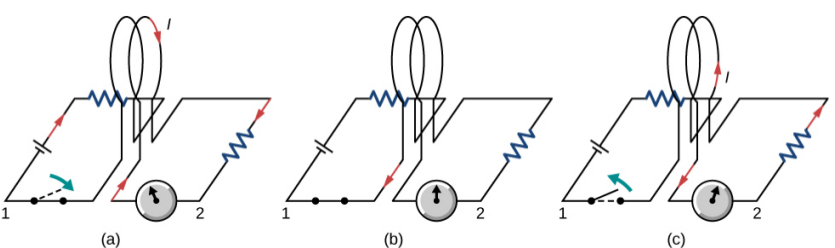
\includegraphics[width=0.6\textwidth]{figures/farad2.png}
\caption{\label{fig:1} The prototypical experiment that reveals Faraday's Law.  Connecting an emf to a circuit with a coil induces an emf in a separate circuit with a corresponding coil.}
\end{figure}

\end{document}